\documentclass[a4paper,12pt,fleqn,twoside]{book}
\usepackage[lmargin=2.0cm, rmargin=2.0cm, tmargin=3.0cm, bmargin=3.0cm]{geometry}
\usepackage[portuguese]{babel}
\usepackage[T1]{fontenc}
\usepackage[utf8x]{inputenc}
\usepackage{amsmath, amsthm, amssymb}
\usepackage{graphicx}
\usepackage{epstopdf}
\usepackage[colorlinks,linkcolor=black,citecolor=black]{hyperref}
\usepackage[sc]{mathpazo}
\usepackage{indentfirst}
\usepackage{setspace}
\usepackage{subfigure}
\usepackage{listings}
\usepackage{lastpage}
\usepackage{float}
\usepackage{hyphenat}
\usepackage{soul} % para usar o \hl 

\usepackage[backend=biber, style=abnt]{biblatex}
\addbibresource{bancoref.bib}

\makeglossary
%\pagestyle{myheadings}
%\setcounter{secnumdepth}{4}
%\setcounter{tocdepth}{4}

% configuração do ambiente de dedicatória
\newenvironment{dedication}{\bgroup\par\noindent\textbf{Dedicatória}\par%
	\[}{\]\egroup}

\begin{document}
	
	\thispagestyle{empty}
	\title{\Huge \textbf{Condução de Calor:}  \\ \huge Aplicações das Funções de Green em Problemas de Engenharia}
	\author{Gilmar Guimarães; Ana P. Fernandes \\ Eduardo O. Peixoto, Sidney R. Silveira}
	%\frontmatter
	\maketitle
	
	% dedicatória
	\thispagestyle{empty}
	\begin{dedication}
		\text{Dedicado ao Prof. James V. Beck}
	\end{dedication}
	
	\pagenumbering{arabic}
	% sumário, lista de figuras e tabelas
	\thispagestyle{empty}
	\tableofcontents
	\thispagestyle{empty}
	\listoffigures
	%\listoftables
	%\mainmatter
	
	%prefácio
	\thispagestyle{empty}
	\chapter*{Prefácio}

	O entendimento das trocas térmicas que ocorrem na natureza e a sua consequente aplicação em problemas de engenharia é a grande motivação do desenvolvimento deste texto. O uso das funções de Green como ferramenta para a solução de problemas  de condução de calor torna-se um instrumento valioso para engenheiros, físicos e matemáticos na solução dos mais variados problemas. Textos clássicos e indispensáveis na literatura como \textcite{carslaw1959}, \textcite{arpaci1966}, \textcite{ozisik1993}, \textcite{beck2010}, \textcite{beck1985} são a base dos fundamentos encontrados aqui e serão constantemente referenciados e recomendados ao longo deste texto. São duas as motivações no desenvolvimento deste texto:
		
	A primeira reflete o objetivo de reunir em um texto os fundamentos de condução de calor, algumas de sua particularidades e, principalmente, fornecer ao profissional ou estudante de engenharia, ferramentas matemáticas poderosas para a solução dos mais variado problemas envolvendo a condução de calor. Ou seja, o contato com o desenvolvimento das soluções analíticas presentes nos textos clássicos, são aqui desenvolvidos de forma a serem implementados numericamente em algoritmos construídos sobre uma plataforma pública como a linguagem Python. As soluções unidimensionais analíticas ou híbridas são detalhadas de forma a permitir que o texto, juntamente com o software disponível possa auxiliar no desenvolvimento de soluções particulares desejadas.
		
	O segundo objetivo traz ao leitor o contato com problemas práticos de engenharia ao abordar a transferência de calor em processos de fabricação como usinagem ortogonal, processos de soldagem, fontes móveis, bio-transferência de calor e investigação de propriedades térmicas. A aplicação de técnicas de problemas inversos usando o conceito de função transferência baseadas em funções de Green dá ao usuário deste texto o entendimento e as ferramentas necessárias para a solução de problemas de engenharia mais complexos.

	Novamente, a força e a contribuição deste texto está intimamente ligado ao uso da plataforma digital e das soluções fundamentais de problemas mais simples até problemas mais complexos que envolvem a condução de calor.
	
	\hl{Colocar uma trajetória das pesquisas no TCME}

	\printbibliography[heading=subbibliography]
	\thispagestyle{empty}
	%\section*{Estrutura do Livro}
	%
	%\cite{beck1985inverse}
	%O Capítulo 1 apresenta os conceitos básicos e fundamentais da condução de calor. Recomenda-se fortemente que o leitor acesse quando necessário os textos de \citet{Carslaw1959ConductionSolids},\cite{Arpaci1966ConductionTransfer}, \cite{Ozisik1993HeatConductionb},\cite{Beck2010HeatFunctions}. No capítulo 2 e 3 são introduzidos a formulação, a obtenção da solução da equação da difusão de calor usando-se as técnicas de funções de Green e o procedimento para a obtenção dessas funções de forma detalhada e direta. Os textos excepcionais de \cite{Ozisik1993HeatConduction} e \cite{Beck2010HeatFunctions} são usados como base e com certeza devem ser consultados para maiores aprofundamentos.
	%Soluções fundamentais, unidimensionais e transientes são apresentadas no Cap. 4.
	%No Capítulo 5 são introduzidas a metodologia para a obtenção de soluções de problemas bi e tri-dimensionais, O conceito de verificação intrínseca, introduzido por \cite{Beck2010HeatFunctions} também são apresentados no Cap. 6. Técnicas de obtenção dessas verificações são também detalhadas no Apêndice B através da obtenção de formas fechadas de somatórios presentes nas soluções baseadas em Funções de Green. Este capítulo encerra o que chamamos de Parte 1 que diz respeito aos fundamentos da condução de calor, das funções de Green e da obtenção das soluções fundamentais 1D-transientes.
	%Apresentam-se, a partir do Capítulo 7 diversas aplicações da condução de calor presentes em problemas de engenharia.
	%No capítulo 7 descreve-se a técnica de função transferência baseada em funções de Green TFBGF que será, por sua vez aplicada nos problemas apresentados nos capítulos seguintes.
	%Apresentam-se a aplicação das soluções em problemas térmicos decorrentes de corte ortogonal como a obtenção da solução de problemas inversos envolvendo estimativas de calor na interface de cavaco-peça-ferramenta (Cap. 8), problemas de bio transferência de calor envolvendo domínio de dupla camada (Cap. 9), e problemas envolvendo fontes móveis como a micro-fresagem (Cap. 10).  Conclui-se o texto apresentando técnicas de estimativas de propriedades térmicas usando-se as funções de Green.
	%%	\part*{Parte I}
	%	%\vspace{1cm} 
	%	\section*{Fundamentos, Funções de Green e Soluções fundamentais}
	
	%\include{Resumo_Introd}
	
	% capitulo 1 e referencias
	\thispagestyle{empty}
	\chapter[Fundamentos de condução de calor]{Fundamentos de condução de calor: Equações governantes e condições de contorno}

\section{Fluxo de Calor e Temperatura}

A condução de calor pode ser entendida como a transferência de energia das partículas mais energizadas para as menos energizadas de um determinado corpo. Esta transferência se dá pela interação molecular. Este fenômeno, por sua vez pode acontecer quer o corpo seja sólido, líquido ou gasoso, embora, nos sólidos ela seja mais eficiente. Esta é, portanto, a razão pela qual este texto somente tratará da condução de calor em sólidos.

Assim, em um corpo sólido cuja variação de temperatura esteja presente, a taxa de transferência de calor por condução ocorrerá da região de alta temperatura para a região de baixa temperatura.  Neste texto, a  \textit{transferência de calor} será tratada como taxa de calor dado em Joules por segundo $[J/s]$ enquanto o termo \textit{fluxo de calor} será associado à taxa de calor por unidade de área  $[W/m^2]$. Ambos os termos estão associados à energia vibracional dos átomos e molécula do corpo.

O fluxo de calor não pode ser medido diretamente.  Entretanto, os efeitos do fluxo de calor podem ser sentidos através da observação. Por exemplo, o aquecimento de uma placa exposta ao sol, o derretimento de uma pedra de gelo, o aquecimento de uma panela ao fogo ou ainda o aquecimento da água no interior da panela. São inúmeros os exemplos. A troca de calor por condução foi investigada pelo pesquisador francês Joseph Fourier cuja observação experimental estabeleceu que a taxa  calor por condução através de uma superfície é dada pelo vetor $\vec{q}$ e pode ser escrita como
\begin{equation}\label{eq:vetorFluxoCalor}
	\vec{q}= -kA \frac{\partial{T}}{\partial{x}} \vec{i} 
	-kA \frac{\partial{T}}{\partial{y}} \vec{j}
	-kA \frac{\partial{T}}{\partial{z}} \vec{k} 
\end{equation}
onde o parâmetro $k$ é a condutividade térmica com unidades $W/(m K)$. Em geral, a condutividade térmica pode ser uma função da temperatura. O sinal negativo implica que o fluxo de calor (que sempre flui no sentido da redução da temperatura) será positivo (por convenção) no sentido do crescimento do eixo. Isso ocorrerá em qualquer das componentes nas direções, seja x, y ou z, ou seja 
\begin{equation}\label{eq:componentesFluxoCalor}
	q_x = -kA \frac{\partial{T}}{\partial{x}}; 
	\qquad  q_y = -kA \frac{\partial{T}}{\partial{y}}; 
	\qquad  q_z = -kA \frac{\partial{T}}{\partial{z}}   
\end{equation}
Esta é a lei de Fourier para a condução de calor. A lei de Fourier se aplica a qualquer corpo que seja homogêneo (possua a mesma substância o tempo todo), isotrópico (o calor flui igualmente em qualquer direção) e com tamanho em macroescala (não muito pequeno).

\section{Equação diferencial geral da difusão de calor} 

\subsection{Equação da difusão de calor diferencial em coordenadas retangulares} 

A equação da difusão de calor é obtida nesta seção para corpos isotrópicos cuja condutividade térmica é constante espacialmente. Além disso, $k$ também não varia com a temperatura. Ou sejam trataremos de problemas lineares. O sistema de coordenadas retangulares $(x; y; z)$ é usado. Obtém-se a equação da difusão de calor aplicando-se o princípio da conservação de energia em uma determinada região de estudo.

Observa-se na  Fig.~\ref{fig:balanco} que um corpo em forma de paralelepípedo tem em suas superfícies informações de temperaturas, $T_{1}$, e $T_{2}$, meios fluídos representados por $h$ e $T_{\infty}$ ou fluxo de calor impostos $q''_0$ e $q''_1$. Essas informações, serão abordadas na próxima seção e representam de fato as condições de contorno do problema a ser analisado.

Um caminho visando a obtenção do campo de temperatura no interior de um sólido, é  a aplicação do princípio de conservação de energia nesse corpo. Entretanto, a aplicação desse princípio exige que ele se dê em uma região de estudo (sistema ou volume de controle) cujas propriedades sejam constantes. Assim, considerando que no problema representado pela Fig.~\ref{fig:balanco} existem gradientes de temperatura no corpo, a primeira lei da termodinâmica só poderá ser aplicada se esta região representar um volume de controle infinitesimal. Esse volume infinitesimal está localizado na coordenada $(x, y, z)$ no corpo e possui um volume $dV = dx dy dz$ conforme mostrado na Fig.~\ref{fig:balanco}. 

Nesse caso, considerando um instante $t$ qualquer, ao aplicar-se o balanço de energia, obtém-se
\begin{figure}[ht]
	\centering
	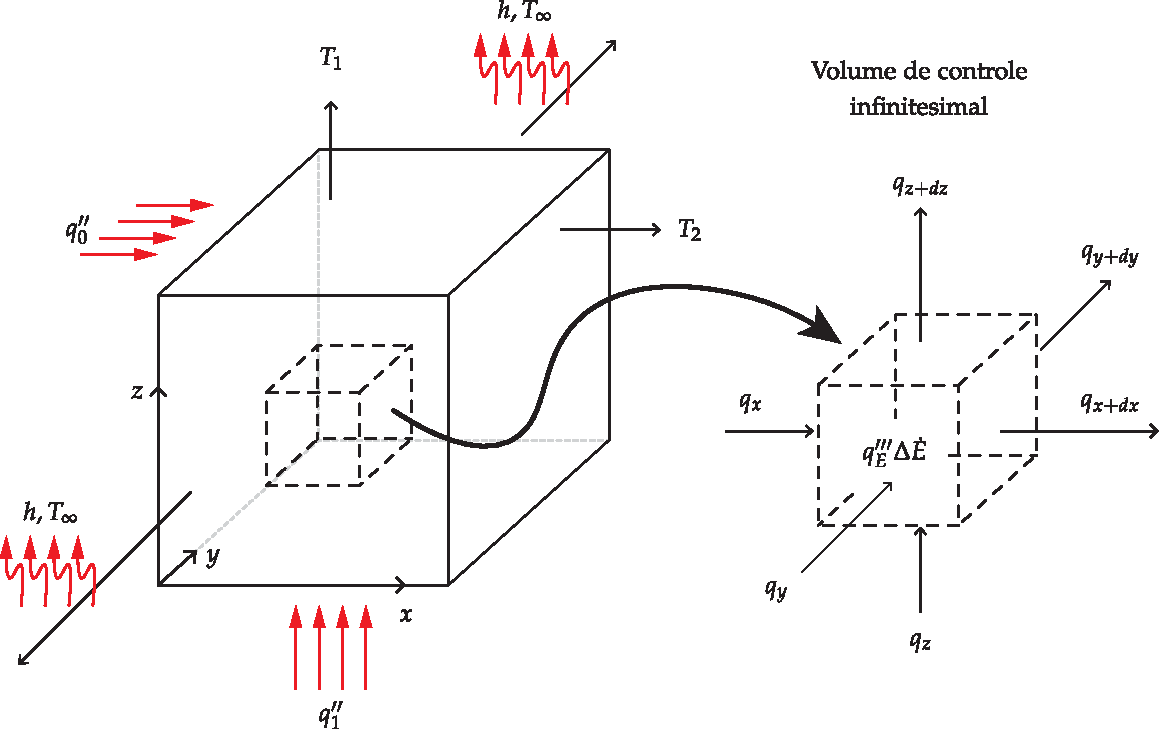
\includegraphics[scale=0.7]{figuras/cap1/balancoEnergia.pdf}
	\caption{Balanço de energia em um volume de controle infinitesimal}	
	\label{fig:balanco}
\end{figure}
\begin{equation}\label{eq:qct}	
	(q_x - q_{x + dx}) +
	(q_y - q_{y + dy}) +
	(q_z - q_{z + dz}) + 
	g(x,y,z,t)  \; dx \; dy \; dz = 
	\rho \; dx \; dy \; dz \; c \; \frac{\partial T}{\partial t}
\end{equation}
Observemos separadamente cada termo da Eq. (\ref{eq:qct}).

\begin{itemize}
	\item Taxa líquida de fluxo de calor entrando e saindo das seis faces do volume de controle.
	\item Consideremos  a convenção de que o fluxo de calor seja positivo nas direções de coordenadas positivas.
	\item A taxa de fluxo líquido de calor é a diferença entre a taxa de fluxo de entrada e a taxa de saída, ou seja
\end{itemize}
\begin{equation}\label{eq:qliq}	 
	q_{\text{liq}} = (q_x - q_{x + dx}) + (q_y - q_{y + dy}) + (q_z - q_{z + dz})
\end{equation}

Observe, por exemplo, que a taxa de fluxo de calor por condução entra no V.C. na face $x$ e sai na face em $x + dx$. Esta taxa é proporcional a área perpendicular a essa direção.  

Nota-se, entretanto, que a posição $x + dx$ corresponde a uma posição muita próxima $x$, porém é de valor simbólico devido o infinitésimo $dx$. Nesse caso, é conveniente que seu cálculo se dê em função da variável exata $x$. Como os pontos situam-se muito próximos, pode-se avaliar a posição $x + dx$ em torno de $x$ usando-se a aproximação em série de Taylor truncada no segundo termo, ou seja, 
\begin{equation}\label{eq:dif1}
	q_{x + dx} = q_x + \frac{\partial q_x}{\partial x} dx 
\end{equation}
\begin{figure}[!ht]
	\centering
	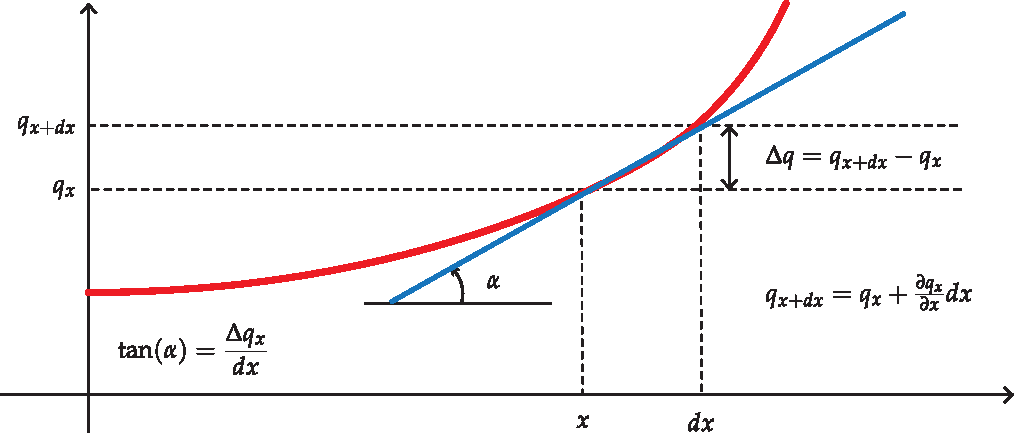
\includegraphics[scale=0.9]{figuras/cap1/aproximacaoTaylor.pdf}
	\caption{Aproximação de Taylor}
	\label{fig:Taylor}
\end{figure} 
A Figura~\ref{fig:Taylor} representa geometricamente esta aproximação, cujo valor de $\partial q_x /\partial x$ tende exatamente ao valor da derivada no ponto $x$ da curva dada pela funçao $q_x$. Assim, analogamente pode-se escrever para as direções $y$ e $z$
\begin{equation}\label{eq:dif2}
	q_{y + dy} = q_y + \frac{\partial q_y}{\partial y} dy  \qquad \text{e}
\end{equation}
\begin{equation}\label{eq:dif3}	
	q_{z + dz} = q_z + \frac{\partial q_z}{\partial z} dz 
\end{equation}

Substituindo as Eqs.(\ref{eq:dif1}),  (\ref{eq:dif2}) e (\ref{eq:dif3}) na Eq. (\ref{eq:qliq}) obtém-se
\begin{equation}
	q_{\text{liq}} =
	- \frac{\partial q_x}{\partial x} dx 
	- \frac{\partial q_y}{\partial y} dy 
	- \frac{\partial q_z}{\partial z} dz 
\end{equation}

Substituindo a definição de cada componente de taxa de fluxo de calor por condução das pelas Eqs.~\ref{eq:componentesFluxoCalor} em suas respectivas direções obtém-se

\begin{equation}
	q_{\text{liq}}=
	- \frac{\partial}{\partial x} \left( - k A_x \frac{\partial T}{\partial x} \right) 
	- \frac{\partial}{\partial y} \left( - k A_y \frac{\partial T}{\partial y} \right)  
	- \frac{\partial}{\partial z} \left( - k A_z \frac{\partial T}{\partial z} \right)   
\end{equation}
onde $A_x, A_y, A_z$ representam as áreas perpendiculares às respectivas direções $x, y, z$. Portanto, pode-se escrever
\begin{equation}\label{eq:Fourierdif1}
	q_{\text{liq}}=
	- \frac{\partial}{\partial x} \left( - k\;dy\;dz \frac{\partial T}{\partial x} \right)  
	- \frac{\partial}{\partial y} \left( - k\;dx\;dz \frac{\partial T}{\partial y} \right)  
	- \frac{\partial}{\partial z} \left( - k\;dx\;dy \frac{\partial T}{\partial z} \right)  
\end{equation}

Apresentam-se no final desta capítulo algumas observações sobre a Lei de Fourier. Considerações sobre o sinal negativo, a sua aplicação em meios macroscópio e aspectos microscópicos bem como as características da condutividade térmica em meios isotrópicos e anisotrópicos.

\textbf{Taxa de geração de energia.} A geração de energia é a energia que afeta o temperatura em todo o volume do corpo. Distingue-se da energia que entra no corpo através dos limites de suas superfícies. A geração de energia pode vir do aquecimento da resistência elétrica dentro do corpo (Efeito Joule), da reação de alguns elementos químicos (por exemplo, o concreto gera calor durante a cura) ou da absorção de radiação (nuclear, micro-ondas ou outra energia eletromagnética). A geração de energia pode variar de um ponto a outro no interior do corpo assim como pode variar com o tempo. A geração de energia também pode ser simplesmente igual a zero. É dado, nesse texto, o símbolo $g(x, y, z, t)$ com unidades $W/m^3$ (taxa de geração de energia por unidade de volume). Assim, considerando o volume de controle infinitesimal tem-se,	
\begin{equation}
	\label{eq:qg}	
	\text{(Taxa de geração de energia)}=g(x,y,z,t) \;dx \;dy \;dz
\end{equation}

\textbf{Taxa de armazenamento de energia.} Uma mudança no armazenamento de energia é definida por $c \Delta T$ para corpos sólidos. Aqui $c$ é o calor específico, J/(kg K), e $\Delta T$ é a variação de temperatura. A taxa de armazenamento de energia específica (por unidade de massa) é dada pela derivada temporal $c(\partial T / \partial t)$. A derivada parcial no tempo é usada porque $T$ também depende da posição $(x,y,z)$. Multiplique a taxa de variação temporal da energia interna específica pela densidade e pelo volume para obter Watts: 
\begin{equation}\label{eq:qct1}	
	\text{(Taxa de armazenamento de energia)} = \rho c \; \frac{ \partial T} {\partial t} \;dx \;dy \;dz
\end{equation}
Assim, substituindo a Eq.(\ref{eq:Fourierdif1}) na equação de energia ( Eq. \ref{eq:qct}) obtém-se 

\begin{equation}\label{eq3Da}
	\frac{\partial}{\partial x} \left(k\frac{\partial T}{\partial x}\right) + 
	\frac{\partial}{\partial y} \left(k\frac{\partial T}{\partial y}\right) + 
	\frac{\partial}{\partial z} \left(k\frac{\partial T}{\partial z}\right) + 
	g(x,y,z,t) = \rho c \frac{\partial T}{\partial t}  
\end{equation}	
e no caso especial em que a condutividade térmica não depende da posição (meios isotrópicos) obtém-se
\begin{equation}\label{eq3Db}
	\frac{\partial^2 T}{\partial x^2} +
	\frac{\partial^2 T}{\partial y^2} + 
	\frac{\partial^2 T}{\partial z^2} = 
	\frac{1}{\alpha} \frac{\partial T}{\partial t}  
\end{equation}
onde $\alpha = k/(\rho c)$ é a difusividade térmica $[m^2/s]$.

\subsection{Outros sistemas de coordenadas}

A equação da energia pode ser aplicada em outros sistemas de coordenadas ortogonais como  os sistemas cilíndrico e esférico apresentados nas Figs.~\ref{fig:coordCilindricas}-\ref{fig:coordEsfericas}.

Uma forma direta de se obter a Equação da Difusão em outras coordenadas é a aplicação da equação de Fourier em sua forma vetorial na equação da energia.

Assim, se a forma vetorial da lei de Fourier é dada por
\begin{equation}\label{eq:Fourier0}
	\mathbf{q} = - k \nabla T  
\end{equation}
onde $\nabla T$ é o gradiente de temperatura e $\mathbf{q}$ é o vetor de fluxo de calor.

Uma forma vetorial da equação de energia que é independente do sistema de coordenadas pode ser dada por
\begin{equation}\label{eq:Fourier}
		- \nabla \cdot \mathbf{q} + g(\mathbf{r},t) = \rho c \frac {\partial T} {\partial t}
\end{equation}
onde $\nabla \cdot \mathbf{q}$ é a divergência do fluxo de calor. A equação da energia em qualquer sistema dado pode ser encontrado substituindo a forma correta da divergência e operadores de gradiente para esse sistema de coordenadas específico. Para uma derivação mais detalhada, consulte \textcite[p. 36]{ozisik1993}.

\subsubsection{Sistema de Coordenadas Cilíndricas}
	
No sistema de coordenadas cilíndricas mostrado na Fig.~\ref{fig:coordCilindricas} a equação da energia é dada por
	
\begin{figure}[ht]
	\centering
	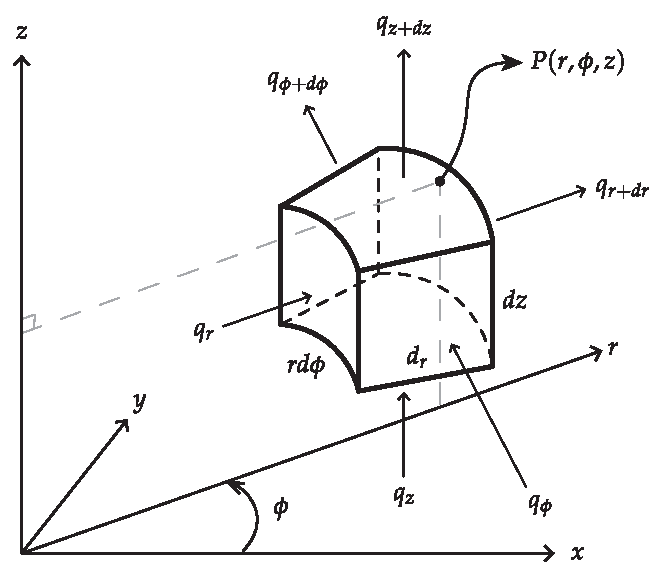
\includegraphics[scale=.9]{figuras/cap1/coordenadasCilindricas.pdf}
	\caption{Sistema de coordenadas cilíndricas e representação do volume de controle  infinitesimal}
	\label{fig:coordCilindricas}
\end{figure}
\begin{equation}\label{eq3Dcila}
	\frac{1}{r}	\frac{\partial}{\partial r} \left(kr\frac{\partial T}{\partial r}\right) +
	\frac{1}{r^2} \frac{\partial}{\partial \phi} \left(k\frac{\partial T}{\partial \phi}\right) + \frac{\partial}{\partial z}\left(k\frac{\partial T}{\partial z}\right) + g = 
	\rho c \frac{\partial T}{\partial t}  
\end{equation}	
	
Considerando $k$ constante obtém-se,
\begin{equation}\label{eq3Dcilb}
	\frac{\partial ^2T}{\partial r^2} + 
	\frac{1}{r} \frac{\partial T}{\partial r} + 
	\frac{1}{r^2} \frac{ \partial ^2T} {\partial \phi ^2} +
	\frac{\partial ^2T}{\partial z^2} + \frac{g}{k} = 
	\frac{1}{\alpha} \frac{\partial T}{\partial t}  
\end{equation}	
	
\subsubsection{Sistema de Coordenadas esféricas}
	
Analogamente, no sistema de coordenadas esféricas mostrado na Fig.~\ref{fig:coordEsfericas}, a equação da energia é dada por
\begin{figure}[ht]
	\centering
	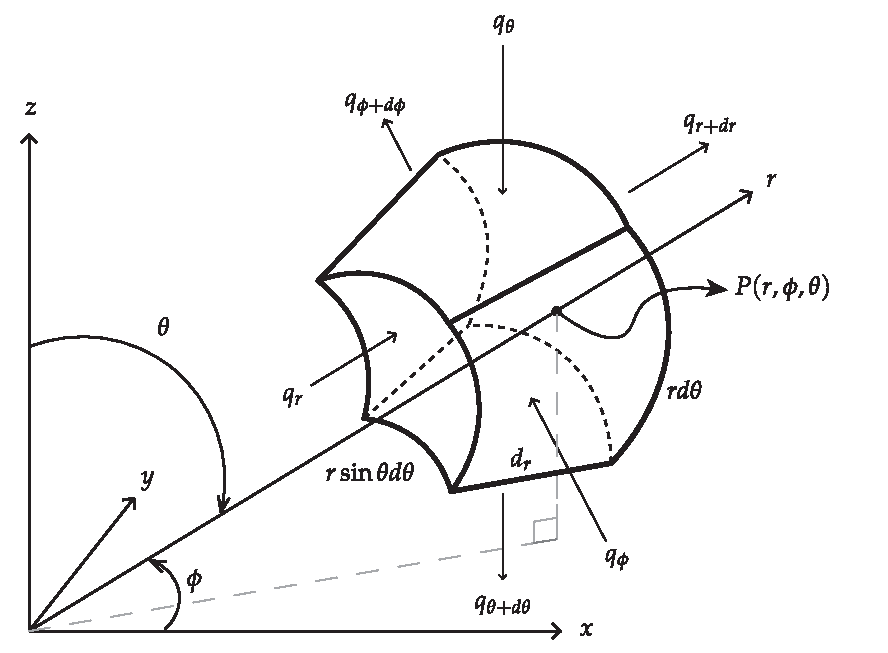
\includegraphics[scale=.9]{figuras/cap1/coordenadasEsfericas.pdf}
	\caption{Sistema de coordenadas esféricas e representação do volume de controle infinitesimal }
	\label{fig:coordEsfericas}
\end{figure} 

\begin{equation}\label{eq3Desfa}
	\frac{1}{r^2} \frac{\partial}{\partial r} 
	\left(kr^2\frac{\partial T}{\partial r}\right) +
	\frac{1}{r^2\sin\theta} \frac{\partial}{\partial\theta} 
	\left(k\sin\theta\frac{\partial T}{\partial\theta}\right) +
	\frac{1}{r^2\sin\theta} \frac{\partial}{\partial\theta} 
	\left(k\sin^2\theta\frac{\partial T}{\partial\phi}\right) + 
	g = \rho c \frac{\partial T}{\partial t}  
\end{equation}	

Similarmente, se $k$ não varia com a posição, obtém-se
\begin{equation}\label{eq3Desfb}
	\frac{1}{r} \frac{\partial^2\left(rT\right)}{\partial r^2} +
	\frac{1}{r^2\sin\theta} \frac{\partial}{\partial\theta}
	\left(\sin\theta\frac{\partial T}{\partial\theta}\right) + 
	\frac{1}{r^2\sin^2\theta}\frac{\partial^2 T}{\partial\phi^2} + 
	\frac{g}{k} = \frac{1}{\alpha}\frac{\partial T}{\partial t}  
\end{equation}
	
\subsection{Condições particulares}
Este curso trata de soluções para a equação de energia conforme elas se aplicam a problemas de engenharia e física. As soluções únicas de cada problema  são estabelecidas pela solução geral aplicando-se as condições de contorno específicas, ou seja, o valor da temperatura (ou sua derivada) nos limites do corpo sólido. A combinação da equação de energia, das condições de contorno específicas e da condição inicial é chamada de problema de valor de contorno. A maior parte deste livro trata de corpos com geometria que possam ser descritos por coordenadas ortogonais. Ou seja, cujos limites estejam localizados onde uma coordenada é uma constante.
	
O número de condições de contorno para um problema de valor de contorno depende da forma da equação de energia e da geometria do sistema em consideração. Por exemplo, a equação de energia bidimensional no sistema de coordenadas retangulares,
\begin{equation}\label{eq2D}
	\frac{\partial ^2T}{\partial x^2} +
	\frac{\partial ^2T}{\partial y^2} + 
	\frac{g(x,y,z,t)}{k} = \frac{1}{\alpha} \frac{\partial T}{\partial t}  
\end{equation}
requer cinco condições: duas para cada um dos limites em $x$ e $y$ e uma condição inicial. As condições de contorno normalmente têm a forma	
\begin{equation}
		k_i \frac{ \partial T} {\partial \eta_i}  +h_i T =  f_i (r_i,t)   
\end{equation}
onde todas as quantidades são avaliadas no limite $i \; esimo$. Aqui $r_i$ é a localização do limite $i \; esimo $ em um sistema de coordenadas específico e $\eta_i$ é o vetor normal da unidade externa no limite. 

As condições iniciais têm a forma
\begin{equation}
	T(r_i, t=0) = F(r_i)   
\end{equation}

As condições de contorno e as condições iniciais são discutidas em detalhes na próxima seção.

\section{Condições de contorno e condição inicial}	

\subsection{Condição de contorno do primeiro tipo}
A Figura \ref{fig:ccTemperaturaPrescrita} apresenta a condição de contorno, chamada do \textit{primeiro tipo}, em que a temperatura da superfície é conhecida. No exemplo apresentado, a temperatura $T_s$ é conhecida e portanto tem-se uma temperatura prescrita. Em alguns textos clássicos, esta condição é também chamada de condição de \textit{Dirichilet}.
\begin{equation}\label{eq:q01}
	T(x=0,t) = T_s 
\end{equation}

\begin{figure}[H]
	\centering
	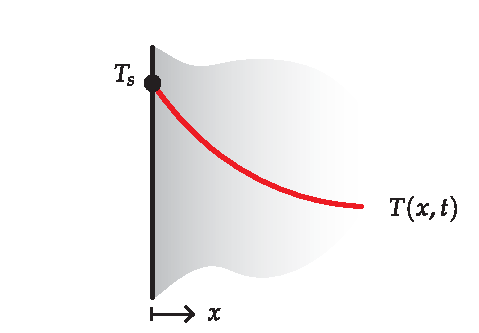
\includegraphics[scale=1]{figuras/cap1/ccTemperaturaConstante}
	\caption{Condição de contorno do primeiro tipo: temperatura prescrita, $T_s$}
	\label{fig:ccTemperaturaPrescrita}
\end{figure}

\subsection{Condição de contorno do segundo tipo}
A Figura \ref{fig:ccFluxoCalor} por sua vez se refere à condição de contorno do \textit{segundo tipo}, sendo nesse caso, conhecido o fluxo de calor no respectivo contorno. Como a informação direta da temperatura não está disponível, a informação desejada para a solução da equação diferencial deve ser obtida através de um balanço de energia na respectiva superfície, ou seja
\begin{equation}\label{eq:q1}
+ q''_s A - q_n = 0  
\end{equation}
Logo,
\begin{equation}\label{eq:q2}
q_n = -k A\left.{\frac{\partial{T}}{\partial{x}}}\right|_{x=0} = q''_s A 
\end{equation}
ou seja,
\begin{equation}\label{eq:q3}
-k\left.{\frac{\partial{T}}{\partial{x}}}\right|_{x=0} = q''_s  
\end{equation}
\begin{figure}[H]
	\centering
	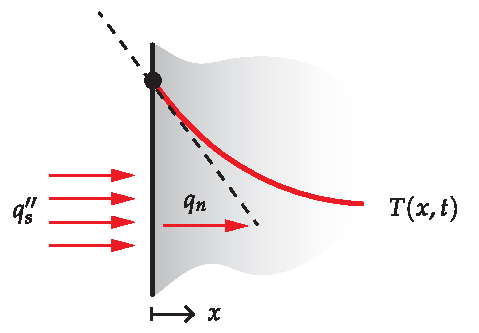
\includegraphics[scale=1]{figuras/cap1/ccFluxoConstante}
	\caption{Condição de contorno do segundo tipo: fluxo de calor prescrito, $q''_0$}
	\label{fig:ccFluxoCalor}
\end{figure}

Caso a superfície esteja isolada termicamente (\hl{fronteita adiabática}), como mostra a Fig.~\ref{fig:ccIsolado}, então pode-se escrever
\begin{equation}\label{eq:q4}
-k\left.{\frac{\partial{T}}{\partial{x}}}\right|_{x=0} =0
\end{equation}

\begin{figure}[H]
	\centering
	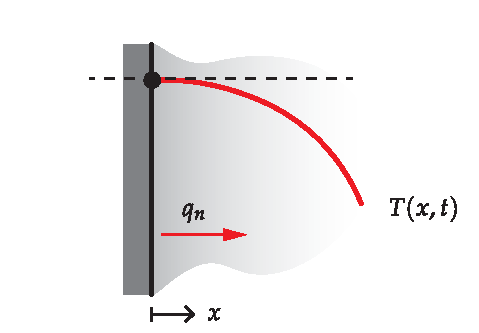
\includegraphics[scale=1]{figuras/cap1/ccAdiabatica}
	\caption{Condição de contorno do segundo tipo: isolado}
	\label{fig:ccIsolado}
\end{figure}

Em alguns textos clássicos, esta condição é também chamada de condição de \textit{Neumann}.

\subsection{Condição de contorno do terceiro tipo}
A condição de contorno do terceiro tipo representada pela Fig.~\ref{fig:ccConveccao} diz respeito à superfície estar exposta a um meio convectivo. 

Nesse caso, um balanço de calor na superfície é escrito como
\begin{equation}\label{eq:q5}
+ q_h - q_n = 0 \Rightarrow q_n = q_h \qquad \text{e}
\end{equation}
\begin{equation}\label{eq:q6}
	-k\left.{\frac{\partial{T}}{\partial{x}}}\right|_{x=0} 
	= h A (T_{\infty} - T(x=0,t))
\end{equation}

\begin{figure}[H]
	\centering
	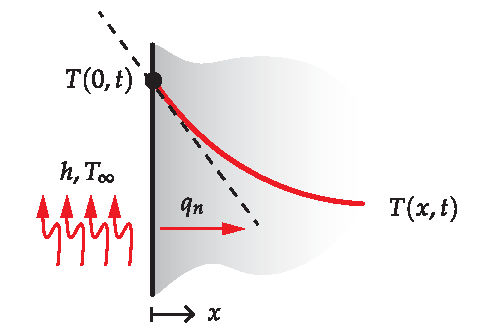
\includegraphics[scale=1]{figuras/cap1/ccConveccao}
	\caption{Condição de contorno do terceiro tipo: face exposta a um meio convectivo}
	\label{fig:ccConveccao}
\end{figure}

Em alguns textos clássicos, esta condição é também chamada de condição de \textit{Robin} ou condição convectiva. 

É importante destacar que ao se aplicar o balanço de energia na superfície, o sinal $+$ indica que a taxa de calor chega na superfície, enquanto o sinal $-$ indica que a taxa de calor deixa a superfície. Como o balanço de energia na superfície, não envolve nenhum fenômeno volumétrico, este balanço sempre será nulo, independente se o problema analisado em questão for transiente ou não.

\section{Notas: A Lei de Fourier e a Condutividade Térmica}

\subsection{Lei de Fourier}
Uma importante observação diz respeito ao sinal negativo da lei de Fourier. Como a taxa de calor por condução é um vetor, ela possui módulo, sentido e direção.

A taxa de calor por condução é igual a
\begin{equation}\label{eq:q7}
- k A \left.{\frac{\partial{T}}{\partial{x}}}\right|_{x=0} 
\end{equation}
e sua direção é sempre perpendicular à superfície isotérmica. 

Já o sentido da taxa de fluxo de calor é sempre o da temperatura maior para a temperatura menor.

Entretanto, uma vez definido uma convenção para o sinal positivo da taxa de fluxo de calor, por exemplo, $q \geq 0$ no sentido positivo do crescimento da direção \;x, o cálculo do gradiente de temperatura sempre produzirá um sinal negativo, independente da escolha da coordenada. Este fato é melhor observado na  Fig.~\ref{fig:sinal}.

\begin{figure}[H]
\centering
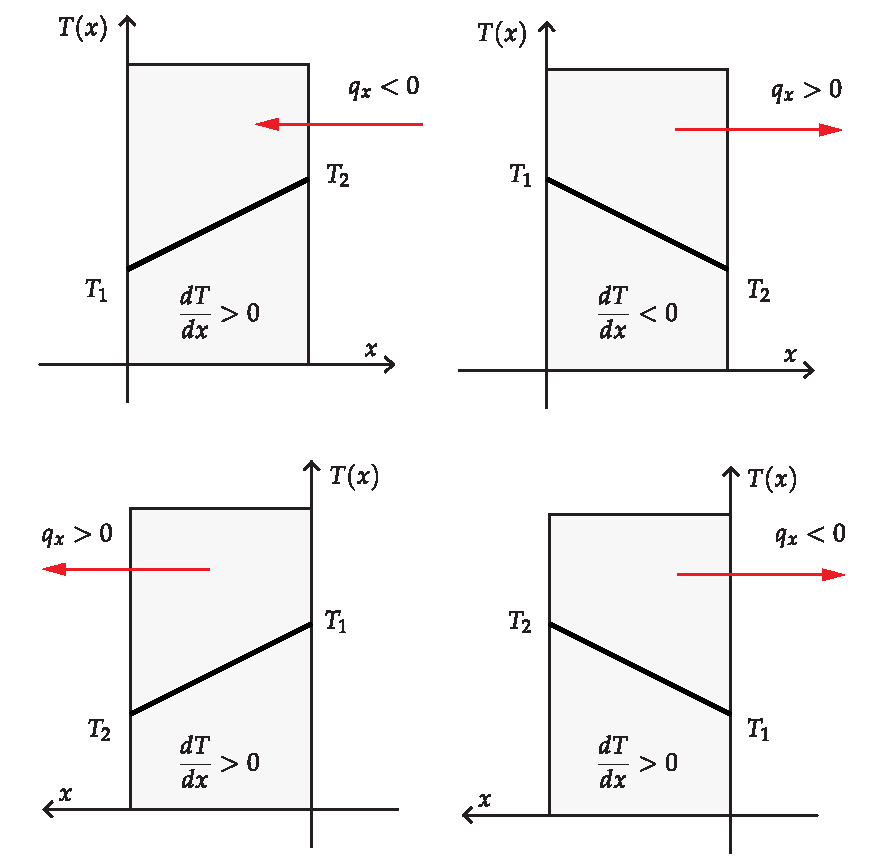
\includegraphics[scale=0.8]{figuras/cap1/fluxo.pdf}
\caption{Convenção do sinal negativo da Lei de Fourier, mudar o sinal da derivada na terceira figura}
\label{fig:sinal}
\end{figure}

Assim, o sinal $-$ é imposto na lei de Fourier para tornar o fluxo de calor uma quantidade positiva na direção da coordenada positiva (ou seja, oposta ao gradiente de temperatura).

Determinar a direção real do fluxo de calor é muitas vezes trivial para problemas unidimensionais (1D). Problemas multidimensionais e notavelmente problemas transitórios, podem apresentar dificuldade considerável em determinar a direção dos termos de fluxo de calor local. Adesão à convenção de sinais para a Lei de Fourier evitará tais dificuldades de determinação de fluxo, o que é útil na contexto de conservação geral de energia para um determinado problema de transferência de calor.

\subsection{Condutividade Térmica}
Dada a dependência direta do fluxo de calor na condutividade térmica via Lei de Fourier, a condutividade térmica é uma propriedade importante na análise da condução de calor. Existe uma ampla variedade de condutividades térmicas de vários
materiais de engenharia. Geralmente, os valores mais altos são observados para metais puros e os menores valores por gases e vapores, com os materiais isolantes amorfos e líquidos inorgânicos com condutividades térmicas intermediárias. 

Para fornecer uma noção da ordem de grandeza da condutividade térmica de diferentes materiais, a Figura \ref{fig:escalacondutividade} apresenta a faixa típica de valores para diversos materiais.

\begin{figure}[H]
\centering
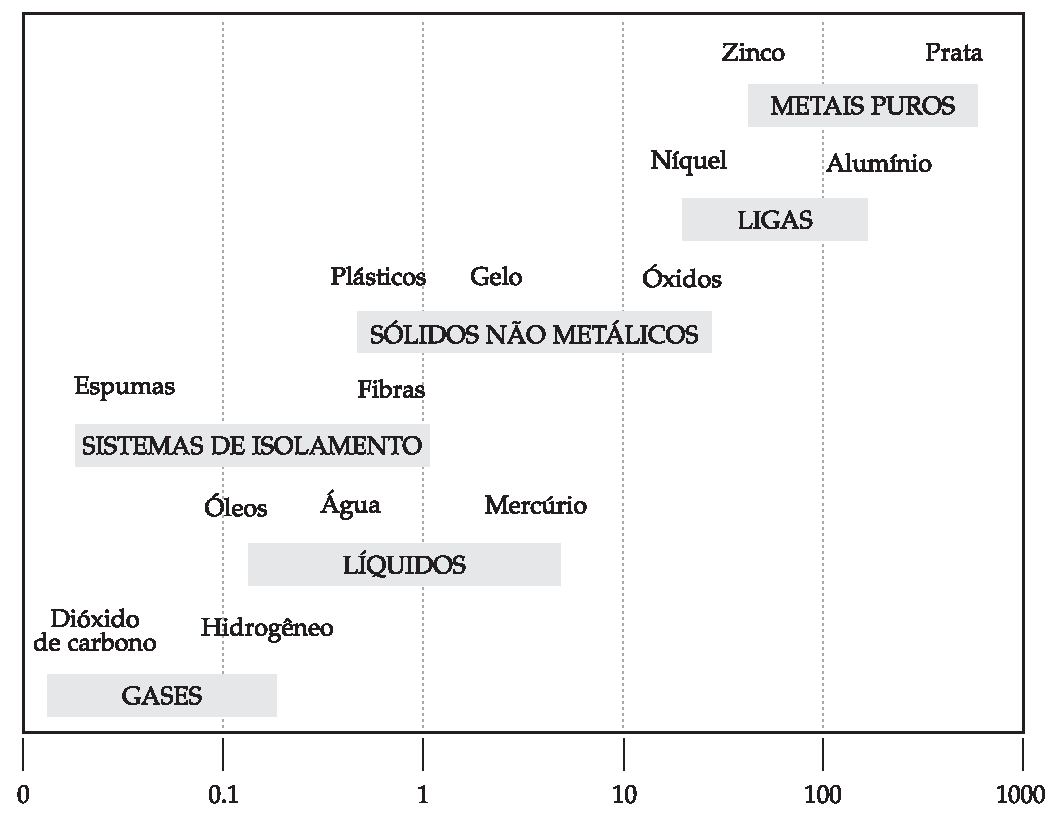
\includegraphics[scale=1]{figuras/cap1/condutividade.pdf}
\caption{Condutividade térmica ($W/mK$), adaptado Incropera.}
\label{fig:escalacondutividade}
\end{figure}

A condutividade térmica também varia com a temperatura e pode mudar com orientação para materiais não isotrópicos. Para a maioria dos metais puros, a condutividade térmica diminui com o aumento da temperatura, enquanto para os gases ela aumenta com o aumento da temperatura. Para a maioria dos materiais isolantes aumenta com o aumento temperatura. 

Uma compilação abrangente de condutividades térmicas de materiais pode ser encontrada nas referências \textcite{arpaci1966, ozisik1993}.

\printbibliography[heading=subbibliography]

	\chapter[Funções de Green]{Funções de Green: Obtenção da equação solução em termos de funções de Green}\label{FG}

\section{Vantagens do Método de Funções de Green}
As funções de Green (FG) são uma ferramenta poderosa na aplicação a soluções de problemas lineares de condução de calor. \textcite{beck2010} citam algumas dessas vantagens no tratamento desses problemas:

\textbf{1.} A primeira vantagem diz respeito a flexibilidade dessas funções, fato que as tornam extremamente poderosas.

A mesma FG pode ser usada para problemas de condução de calor diferentes condições de contorno, desde que se trate de uma mesma geometria. Ou seja, independente das condições de contorno, dos termos de geração de energia volumétrica ou das condições iniciais do campo de temperatura, existe somente uma função de Green relacionada ao problema físico. Ainda, essa função de Green se refere e pode ser obtida de um problema físico de mesma geometria, porém considerando-se todas as condições de contorno homogêneas.

\textbf{2.} Uma segunda vantagem do método GF é o procedimento de solução sistemática.

Muitas GFs estão disponíveis na literatura e encontram-se tabuladas. Por exemplo, o livro  \textcite{beck1993} e \textcite{beck2010} apresentam várias funções de Green para a grande maioria de problemas envolvendo coordenadas retangulares, cilíndricas e esféricas. Assim, a maioria dessas funções não precisam necessariamente serem obtidas. As autofunções e autovalores também estão disponíveis. O uso dessas funções tabeladas economizam esforço e reduzem a possibilidade de erro. Problemas bidimensionais e tridimensionais podem ser construídos a partir das funções de Green unidimensionais. Este texto, apresenta todas as funções de Green em coordenadas retangulares, expressas matematicamente e implementadas numericamente a partir do estabelecimento de um problema específico. A construção em forma de bloco permite facilmente o uso de problemas mais gerais. A verificação intrínseca dessas soluções permitem também a ganho de confiança nos resultados obtidos a partir das implementações numéricas.

\textbf{3.} Uma terceira vantagem é que GFs bidimensionais e tridimensionais podem ser encontradas, para casos transientes, por simples multiplicação de GFs unidimensionais para o sistema de coordenadas retangulares para a maioria das condições de contorno consideradas em neste livro.  As limitações na obtenção das Funções de Green multidimensionais deve-se a exigência da linearidade da equação diferencia e ainda que o corpo deve ser espacialmente uniforme (homogêneo) e a geometria deve ser ortogonal.  

O uso da multiplicação de FG unidimensionais para a obtenção de FG bi e tridimensional resulta em uma grande simplificação nas soluções de problemas de condução de calor fornecendo um formas compactas para catalogar funções de Green desses casos. Este texto apresenta uma abordagem de parte destes problemas.

\textbf{4.} Uma quarta vantagem é que existem formas alternativas para a obtenção da equação solução em termos FG. Estas formas, chamadas de formas fechadas melhoram a convergência dessas funções e diminuem o número de termos das séries envolvidas, que por sua vez, necessitam, dependendo do problema de um número grande de termos.

\textbf{5.} A quinta vantagem do método FG é a sua verificação intrínseca. Ou seja, as soluções construídas a partir de FG contêm em si os meios para verificar se os valores numéricos calculados estão corretos. Como um exemplo de verificação intrínseca, quando uma solução transiente contém um termo estacionário e um termo transiente, no tempo inicial existe uma região na qual esses termos necessariamente devem somar zero. Assim, essa região esses termos são verificados, um contra o outro.

\textbf{6.} A sexta vantagem do método GF é o particionamento do tempo, que pode reduzir o número de termos da série necessários para obter uma solução precisa. A partição de tempo é um método geral que surge naturalmente do método FG e pode fornecer valores precisos para temperatura usando apenas alguns termos da série infinita.


\section{A Função Delta de Dirac Delta}

A função Delta de Dirac (às vezes chamada de função impulso unitário) desempenha um papel central no método das funções de Green. Nesta seção, apresentamos a definição da função Delta de Dirac em termos das propriedades que são mais importantes para o desenvolvimento do método de funções de Green.

Estritamente falando, a função Delta de Dirac é uma função matemática simbólica cuja definição é dada por:

A função Delta de Dirac $\delta (x)$ é definida como zero quando $\delta (x)\neq 0$, e infinita em $x = 0$ de forma que a área sob a função seja unitária.

Algumas das propriedades da função delta de Dirac são dadas por:
\begin{equation*}
    \begin{split}
        \delta(x-x') =  \infty  \qquad & \text{em}  \qquad x = x' \\
        0 \qquad  & \text{em}  \qquad x \neq x'\\ 
        \displaystyle \int_{-\infty}^{\infty} \delta(x-x') dx' & =  1 \\  
        \displaystyle \int_{-\infty}^{\infty} F(x') \delta(x-x') dx' & = F(x) \\  
        \delta(x-x') \qquad & \text{tem unidade de} \; m^{-1} \\ 
        \delta(t-\tau) \qquad & \text{tem unidade de} \; s^{-1} \\
    \end{split}
\end{equation*}

O uso da função Delta de Dirac na concepção de um problema de condução de calor particular é uma ferramenta importante para se entender o significado físico das funções de Green.  A próxima seção aborda este tema.

\section{Temperatura em um corpo unidimensional infinito}
A Figura \hl{xx} apresenta um corpo infinito em um modelo unidimensional, propriedades constante com temperatura inicial $F(x)$ e geração de energia volumétrica $g(x,t)$ (com unidades $W/m^3$) cuja equação governante é dada por
\begin{equation}\label{eq1Da}
    \frac{\partial^2 T}{\partial x^2} + \frac{g(x,t)}{k}  
    = \frac{1}{\alpha}\frac{\partial T}{\partial t}  
\end{equation}
com as condições de contorno 
\begin{equation}\label{eq1Db}
    T(x,0) = F(x)
\end{equation}
\begin{equation}\label{eq1Dc}
    T(x\rightarrow  \pm \infty) = F(x)
\end{equation}

A temperatura T(x,t) que é uma solução para as Eqs. \ref{eq1Da}-\ref{eq1Dc} pode ser obtida formalmente por meio da Equação da solução da difusão de calor em termos de funções de Green como
\begin{equation}\label{eq:solg}
    \displaystyle \theta(x,t) = \int_{x'=0}^{\infty} G(x,t|x',0) F(x')dx' +
    \frac{\alpha}{k}
    \int_{0}^{t}\int_{x'=\infty}^{\infty}G(x,t|x',\tau)g(x',\tau)dx'd\tau
\end{equation}

A obtenção formal da Eq. \ref{eq:solg} será demonstrada para um problema geral, 1D com dimensões finitas transiente, com geração de calor espacial e temporal na próxima seção e sujeito as condições de contorno no homógenas com variação temporal. Assim, para o entendimento físico das funções de Green, considere neste ponto que a Eq.\ref{eq:solg} é solução do problema dado pelas Eqs. \ref{eq1Da}. Esta informação será demonstrada a seguir. No apêndice xx será demonstrado a obtenção da Equação Geral em Termos de Funções de Green.

\section{Duas Interpretações das Funcões de Green}
Existem dois termos integrais na equação solução  Eq.~\ref{eq:solg}, um contendo as condições iniciais $F(x)$ e o outro contendo a fonte de energia volumétrica $g(x,t)$. Cada termo integral pode ser considerado a solução de um problema separado, um causado por $F(x)$ e outro por $g(x,t)$, que são sobrepostos (ou seja, somados) para formar a solução completa. É importante notar que quando $F$ e $g$ são substituídos nas integrais acima, a dependência coordenada assume a forma $F(x')$ e $g(x',\tau)$, associada às variáveis de integração. Este procedimento será melhor explorado na seção \hl{xxx}.

Duas interpretações físicas diferentes de $G(.)$ podem ser encontradas na equação da solução GF. A primeira interpretação física de G(.) é a distribuição de temperatura causada por uma condição inicial particular e a segunda interpretação é a distribuição de temperatura para uma fonte de calor instantânea.

\subsection{Interpretações das Funcões de Green: Condição inicial, F(x)}
A primeira interpretação física está associada ao primeiro termo na Eq.~\ref{eq1Da}
e é a solução $T(x,t)$ para o problema
\begin{equation}\label{eq1Daa}
    \frac{\partial ^2T}{\partial x^2} = \frac{1}{\alpha}\frac{\partial T}{\partial t} 
\end{equation}

\begin{equation}\label{eq1Dbb}
    T(x,0) = F(x)
\end{equation}

Se a distribuição de temperatura inicial for zero em todos os lugares, exceto em $x_0$ onde
exite um distribuição inicial igual a $F'_0$ vezes a função delta de Dirac .

\begin{equation}\label{delt}
    F(x) = F'_0 \delta(x-x_0)
\end{equation}
então a solução das Eqs.~\ref{eq1Daa} e \ref{delt} é
\begin{equation}\label{eq:solTi}
    \displaystyle \theta(x,t) = \int_{x'=0}^{\infty} G(x,t|x',0) F'_0 \delta(x'-x_0)dx'
\end{equation}
ou
\begin{equation}\label{deltfx}
	T(x,t) = F'_0 \; G(x,t|x_0,0)
\end{equation}
e portanto
\begin{equation}\label{deltfx1}
	T(x,t) = G(x,t/x_0,0)
\end{equation}

Isto significa que
\begin{equation}\label{deltfx2}
	G(x,t/x_0,0) =	T(x,t)
\end{equation}


Portanto, a função de Green $G(x,t/x',0)$ pode ser interpretada como sendo a distribuição de temperatura no corpo que resulta da solução de  um problema térmico de dimensões infinitas cuja distribuição inicial é devido o produto de $F'_0$ vezes a função delta de Dirac de onde a magnitude de $F'_0$ é dada por $F'_0= 1 K-m$ (Kelvin-metro). 

As unidades de $G(.)$ é de unidade  $m^{-1}$ assim como a unidade de $\delta(x-x_0)$ também é $m^{-1}$.

\subsection{Interpretações das Funções de Green: Geração de calor}
A segunda interpretação física de uma GF é a temperatura causada por uma fonte de calor instantânea no instante $t_0$ e na posição $x_0$ e de intensidade $H\rho c$.
Para este caso, o termo de geração de energia volumétrica na equação do calor, \ref{eq:solg} torna-se

\begin{equation}\label{deltfx3}
    g(x,t) = H \rho c \delta(x-x_0) \delta(t-t_0)
\end{equation}
onde $H$ tem unidades de $K-m$; $\delta (x-x_0)$ tem unidade de $m^-1$; $\delta(t-t_0)$ tem unidade de $s^-1$; e $\rho c$ tem unidade de $J/m^3/K$.

Essas unidades são consistentes com as do volume de geração de energia $g(x,t)$, que são $W/m^3$. O símbolo $g$ dado pela Eq.~\ref{deltfx3} representa a quantidade de energia que é liberada em $x=x_0$ e em $t = t_0$.

O termo $g(x_0,t_0)$ pode ser visualizado como a energia associada a uma fonte plana aplicada em um instante $t_0$ na direção normal ao eixo $x
$. Pode ser representado, por exemplo, como uma fonte laser (pulsada) sendo liberada em $x = x_0$ e no instante de tempo $t_0$. Para este caso, descreve-se a equação diferencial governante do problema como sendo
\begin{equation}\label{eq1Gx}
    \frac{\partial ^2 T}{\partial x^2} + \frac{H \rho c \delta(x-x_0) \delta(t-t_0)}{k}
    = \frac{1}{\alpha} \frac{\partial T}{\partial t}  
\end{equation}

Para esse problema, a condição inicial é distribuição e temperatura igual  zero, ou seja
\begin{equation}\label{eqinit}
    T(x,t_0) = 0
\end{equation}

Nesse caso, a solução das Eqs.~\ref{eq1Gx} é dada por 
\begin{equation}\label{eq:solg1}
    \theta(x,t) =  + \frac{\alpha}{k}\int_{0}^{t} 
    \int_{x'=-\infty}^{\infty}G(x,t|x',\tau)H \rho c \delta(x'-x_0) \delta(t-t_0) dx'd\tau
\end{equation}

Ou seja,
\begin{equation}\label{eq:solg2}
    \theta(x,t) =  + \frac{\alpha}{k}H \rho c 
    \int_{0}^{t}\int_{x'=-\infty}^{\infty}G(x,t|x',\tau) \delta(x'-x_0) \delta(t-t_0) dx'd\tau
\end{equation}

Portanto,	
\begin{equation}\label{deltfx30}
    T(x,t) = H\;G(x,t/x_0,t_0) 
\end{equation}

como $H=1$,
	
\begin{equation}\label{deltfx4}
    T(x,t) = G(x,t/x_0,t_0)  
\end{equation}
	
ou
\begin{equation}\label{deltfx5}
    G(x,t/x_0,t_0) = T(x,t)
\end{equation}
	
Isso significa que a FG é igual ao aumento de temperatura para a fonte de calor plana instantânea dada pela Eq.~\ref{deltfx5} com $H = 1 K.m$.
	
Essas duas formas alternativas de se pensar sobre GFs transientes são muito importantes.
	
Na primeira interpretação, a FG é igual à temperatura resultante de uma distribuição de temperatura inicial que é zero em todos os lugares, exceto em uma determinada posição $x_0$ cuja magnitude é dada pelo produto da função Delta de Dirac e intensidade de $1 K-m$.
	
Na segunda interpretação, a FG é igual ao aumento de temperatura devido a aplicação de uma fonte plana instantânea de Geração de calor cuja magnitude é dada pelo produto de produto da função Delta de Dirac e de uma intensidade de $K-m$ vezes $\rho c$.	
	
\section{Propriedades comuns às funções de Green transientes}
As propriedades comuns a FG para condução de calor transiente são resumidas a seguir.

1. A FG obedece à soluçao de um problema auxiliar.
	
2. A FG é uma solução do problema de condução de calor com a mesma geometria, e mesmo tipo de condições de contorno do problema original, porém em sua versão homogênea.

3. A FG obedece à relação de causalidade: $G\geq 0$ no domínio $R$ para $t\geq 0$; e, $G = 0$ no domínio $R$ para $t \leq 0 $ 

4. O FG obedece à relação de reciprocidade: $G(x,t/x',\tau)= G(x',-\tau/x,-t)$. 

5. A dependência temporal de $G$ é sempre $t-\tau$ , então uma $FG$ unidimensional pode ser escrita como G(x, x', t -$\tau$).

6. Em coordenadas retangulares, a $FG$  transiente tem unidades de:$ m^{-1} $ para problemas unidimensionais; $ m^{-2} $ para problemas bidimensionais; e $ m^{-3} $ para problemas tridimensionais.
Toda $FG$ é uma solução para uma equação auxiliar com contorno homogêneo condições. 

A  $FG$  é sempre positiva ou nula, porque é a resposta da temperatura causada por um pulso de calor positivo. 
	
A relação de causalidade refere-se à ideia de que  a $FG$  é a resposta no tempo t e localização x para um pulso de calor que ocorre em um instante $\tau$ e na localização $x'$. Em um sistema real (ou causal), não pode haver resposta antes que o pulso de calor ocorra.

A relação de reciprocidade pode ser entendida a partir da equação auxiliar. 

Trocar $x$ e $x'$ na equação auxiliar deixa o sinal do solução inalterada por causa da segunda derivada em relação a $x$. 
Entretanto, trocar $t$ e $\tau$ muda o sinal da solução, devido a primeira derivada em relação a t. A orientação espacial não tem direção preferencial na condução de calor, mas o tempo tem uma direção preferencial.
\section{Dedução da Equação solução em termos das funções de Green}
Inicialmente, escrevemos a equação governante do problema original generalizado
\begin{equation}\label{eqGT}
    \frac{\partial ^2T}{\partial x^2} + \frac{g(x,t)}{k} 
    = \frac{1}{\alpha} \frac{\partial T}{\partial t}  
\end{equation}
sujeito ás condições de contorno
\begin{equation}\label{ccemT}
    k_i \frac{\partial T(x_i,t)}{\partial x}  + h_i T(x_i,t) =  f_i(x_i,t)   
\end{equation}
e à condição inicial
\begin{equation}\label{iniT}
    T(x,0) = F(x)
\end{equation}
	
Suponha um problema auxiliar definido pela versão homogênea do problema original (Eq.~\ref{eqGT}
\begin{equation}\label{eqGG}
    \frac{\partial ^2G}{\partial x^2} + 
    \frac{1}{\alpha} \delta(x-x')\delta(t-\tau) = 
    \frac{1}{\alpha} \frac{\partial G}{\partial t}  
\end{equation}

sujeito ás condições de contorno
\begin{equation}\label{ccemG}
    k_i \frac{ \partial G(x_i,t)} {\partial x}  +h_i G(x_i,t) =  0   
\end{equation}
e à condição inicial	
\begin{equation}\label{iniG}
    G(x,0) = 0
\end{equation}
	
Considerando a reciprocidade
\begin{equation}\label{rec}
    G(x,t/x',t) =  G(x',-\tau/x, -t) 
\end{equation}
então é possível a mudança de variável na função $G(x,t/x',t)$ ou seja
	
\begin{equation}\label{eq1DGtau}
    \frac{\partial^2 G}{\partial x'^2} + 
    \frac{1}{\alpha} \delta(x'-x)\delta(t-\tau) = 
    -\frac{1}{\alpha} \frac{\partial G}{\partial \tau}  
\end{equation}
Observe o sinal negativo na derivada temporal. Como já mencionado, o tempo tem uma direção preferencial. Isto é, ele somente ocorre em um sentido. Nesse caso, como a dependência da  função de Green no tempo é dada por $G(u)$ sendo $u =  t - \tau$, ou $\tau = t - u$ . Assim, uma vez que
\begin{equation}\label{rec3}
    \frac{ \partial u}{\partial t} = 1
\end{equation}
	
\begin{equation}\label{rec4}
    \frac{ \partial u}{\partial \tau} = -1
\end{equation}
então
	
\begin{equation}\label{rec6}
    \frac{\partial G(u)}{\partial u} = 
    \frac{\partial G(u)}{\partial t} \frac{\partial t}{\partial u} = 
    \frac{\partial G(u)}{\partial t}
\end{equation}
porém   	
\begin{equation}\label{rec7}
    \frac{\partial G(u)}{\partial u} = 
    \frac{\partial G(u)}{\partial \tau} \frac{\partial \tau}{\partial u} =
    -\frac{ \partial G(u)}{\partial \tau} 
\end{equation}

Assim, avaliando $T(x,t)$ em $T(x',\tau)$ tem-se equação do campo de temperatura escrita em termos $T(x',\tau)$
\begin{equation}\label{eq1DT1}
    \frac{\partial^2 T}{\partial x'^2} + 
    \frac{g(x',\tau)}{k} 
    = \frac{1}{\alpha} \frac{\partial T}{\partial \tau}  
\end{equation}
multiplicando a Eq. \ref{eq1DT1} por $G(x,t/x',\tau)$ obtém-se
	
\begin{equation}\label{eq1DT2}
    G \times \frac{\partial^2 T}{\partial x'^2} + 
    G \times \frac{g(x',\tau)}{k} = 
    G \times \frac{1}{\alpha}\frac{\partial T}{\partial \tau}  
\end{equation}

Por sua vez, multiplicando a Eq.~\ref{eq1DGtau} por $T(x',\tau)$ obtém-se
\begin{equation}\label{eq1DGtau1}
    T \times \frac{\partial^2 G}{\partial x'^2} + 
    T \times \frac{1}{\alpha} \delta(x'-x)\delta(t-\tau) = 
  - T \times \frac{1}{\alpha} \frac{\partial G}{\partial \tau}  
\end{equation}

Subtraindo a Eq.~\ref{eq1DT2} pela  Eq.~\ref{eq1DGtau1}
\begin{equation}\label{eq1DT3}
    G \frac{\partial^2 T}{\partial x'^2} - 
    T \frac{\partial^2 G}{\partial x'^2} + 
    \frac{G}{k}g(x',\tau) - \frac{T}{\alpha}\delta(x'-x)\delta(t-\tau ) = 
    G \frac{1}{\alpha} \frac{\partial T}{\partial\tau} + 
    T \frac{1}{\alpha} \frac{\partial G}{\partial\tau}  
\end{equation}	

Resta-nos portanto integrar cada membro da Eq.~\ref{eq1DT3} no espaço e no tempo. Ou seja
\begin{equation}\label{eq1DT4}
    G \frac{\partial^2 T}{\partial x'^2} -
    T \frac{\partial^2 G}{\partial x'^2} + 
    \frac{G}{k}g(x',\tau) - \frac{T}{\alpha}\delta(x'-x)\delta(t-\tau) = 
    \frac{1}{\alpha} \frac{\partial(TG)}{\partial\tau} 
\end{equation}	
integrando 

\begin{equation}\label{eq:TGTG1}
    \begin{split}
	\int_{d\tau=0}^{t+\epsilon} d\tau
        \int_{x'=0}^{L} \left(G \frac{\partial^2 T}{\partial x'^2} 
      - T \frac{\partial ^2G} {\partial x'^2} \right)dx' + 
	\frac{1}{k} \int_{d\tau=0}^{t+\epsilon} d\tau \int_{x'=0}^{L} g(x',\tau) G(x,t|x',\tau) dx' - \\
        \frac{1}{\alpha}\int_{x'=0}^{L} \int_{d\tau=0}^{t+\epsilon}T(x',t) \delta(x'-x)\delta(t-\tau) dx' d\tau = 
        \frac{1}{\alpha} \; \int_{x'=0}^{L} dx' \int_{d\tau=0}^{t+\epsilon} \; \frac{ \partial (T \; G)} {\partial \tau} d\tau
    \end{split}
\end{equation}
	
Isolando o terceiro membro esquerdo da Eq.~\ref{eq:TGTG1} temos 
\begin{equation}\label{eq:TGTG2}
    \begin{split}
        \frac{1}{\alpha}\int_{x'=0}^{L} 
        \int_{d\tau=0}^{t+\epsilon}T(x',\tau) \delta(x'-x)\delta(t-\tau) dx' d\tau = 
        \alpha \int_{d\tau=0}^{t+\epsilon} d\tau 
        \int_{x'=0}^{L} \left(G\frac{\partial^2T}{\partial x'^2} - 
        T \frac{\partial^2 G}{\partial x'^2}\right)dx' + \\
        \frac{\alpha}{k} \int_{d\tau=0}^{t+\epsilon} d\tau
        \int_{x'=0}^{L}g(x',\tau)G(x,t|x',\tau) dx' - 
        \int_{x'=0}^{L} dx' 
        \int_{d\tau=0}^{t+\epsilon} \frac{\partial(TG)}{\partial\tau} d\tau 
    \end{split}
\end{equation}

Porém, considerando a propriedade da função Delta de Dirac
\begin{equation}\label{eq:dirac}
    \int_{-\infty}^{\infty} F(x') \delta(x-x') dx' = F(x)
\end{equation}	
o membro esquerdo da Eq.~\ref{eq:TGTG2} se reduz a 
\begin{equation}\label{eq:TGTG3}
    \frac{1}{\alpha}\int_{x'=0}^{L} 
    \int_{\tau=0}^{t+\epsilon}T(x',\tau) \delta(x'-x)\delta(t-\tau) dx' d\tau = 	\frac{1}{\alpha}\int_{x'=0}^{L} T(x',t+\epsilon) \delta(x'-x)dx' 
\end{equation}
e a 
\begin{equation}\label{eq:TGTG4}
    \frac{1}{\alpha}\int_{x'=0}^{L} 
    \int_{\tau=0}^{t+\epsilon}T(x',\tau) \delta(x'-x)\delta(t-\tau) dx' d\tau = 	\frac{1}{\alpha} T(x,t+\epsilon) 
\end{equation}
portanto, isolando $T(x,t)$ têm-se
\begin{equation}\label{eq:TGTG5}
    \begin{split}
        T(x,t)= -\int_{d\tau=0}^{t+\epsilon} \frac{\partial (TG)}{\partial\tau} d\tau +
        \frac{\alpha}{k} 
        \int_{d\tau=0}^{t+\epsilon} d\tau 
        \int_{x'=0}^{L}g(x',\tau)G(x,t|x',\tau) dx' + \\ 
	\alpha \int_{d\tau=0}^{t+\epsilon} d\tau
        \int_{x'=0}^{L} \left(G\frac{\partial ^2T}{\partial x'^2} - T \frac{\partial^2 G}{\partial x'^2}\right)dx'
    \end{split}
\end{equation}

O primeiro termo do lado direito da Eq.~\ref{eq:TGTG5} pode ser escrito como
\begin{equation}\label{eq:TG1}
    \int_{\tau=0}^{t+\epsilon} \frac{\partial(TG)}{\partial \tau} d\tau =
    [TG]_0^{t+\epsilon} = T(x',t+\epsilon) G(t-(t+\epsilon)) - T(x',0) G(x,t/x',0)
\end{equation}
como $T(x,0)$ é a condição inicial do problema original, ou seja $T(x',0)=F(x')$ e ainda	$G(-\epsilon)=0$ então
\begin{equation}\label{eq:xx2}
    [TG]_0^{t+\epsilon} = T(x',t+\epsilon) \times 0 - T(x',0) G(x,t/x',0) = F(x') G(x,t/x',0)				
\end{equation}
ou
\begin{equation}\label{eq:xx3}
    [TG]_0^{t+\epsilon} = - F(x') G(x,t|x',0)	
\end{equation}

Integrando por partes o segundo termo do lado direito da Eq.~\ref{eq:TGTG4} obtem-se
\begin{equation}\label{eq:TGTG51}
        \int_{x'=0}^{L} \left(G\frac{\partial ^2T}{\partial x'^2} -
        T \frac{\partial ^2G}{\partial x'^2}\right)dx' = 
        \left. G{\frac{\partial{T}}{\partial{x}}} \right|^{x'=L}_{x'=0} -\int_{x'=0}^{L}\frac{\partial G}{\partial x'} \frac{\partial T} {\partial x'} dx' - 
	\left. T{\frac{\partial{G}}{\partial{x}}}\right|^{x'=L}_{x'=0} +
        \int_{x'=0}^{L}\frac{\partial T}{\partial x'}\frac{\partial G}{\partial x'}dx'
\end{equation}
ou seja
\begin{equation}\label{eq:TGTG6}
    \int_{x'=0}^{L} 
    \left(G \frac{\partial ^2T} {\partial x'^2} - 
    T \frac{\partial ^2G} {\partial x'^2}\right)dx' = 
    G \left.{\frac{\partial{T}}{\partial{x'}}}\right|^{x'=L}_{x'=0} 
   -T \left.{\frac{\partial{G}}{\partial{x'}}}\right|^{x'=L}_{x'=0}
\end{equation}

Observem que o termo do lado direito da \hl{Eq.} pode ser obtido a partir das condições de contorno do problema original e do problema auxiliar, ou seja se
\begin{equation}\label{eq:ccT}
    \left.{\frac{\partial{T}}{\partial{x'_i}}}\right|_{x'=x_i} =
    \frac{f_i(\tau)}{k_i} - \frac{h_i}{k_i} \left.{T}\right|_{x'=x_i}
\end{equation}
e 
\begin{equation}\label{eq:ccG}
    \left.{\frac{\partial{G}}{\partial{x'_i}}}\right|_{x'=x_i} =
    -\frac{h_i}{k_i} \left.{G}\right|_{x'=x_i}
\end{equation}
então, multiplicando a Eq.~\ref{eq:ccT} por $G$ e a Eq.~\ref{eq:ccG} por $T$ e subtraindo, obtém-se 
\begin{equation}\label{eq:ccTG}
    \left.{G}\right|_{x'=x_i}\left.{\frac{\partial{T}}{\partial{x'_i}}}\right|_{x'=x_i} - 
    \left.{T}\right|_{x'=x_i} \left.{\frac{\partial{G}}{\partial{x'_i}}}\right|_{x'=x_i} = 
    \left.{G}\right|_{x'=x_i} \left( \frac{f_i(\tau)}{k_i} -  \frac{h_i}{k_i} \left.{T}\right|_{x'=x_i}   \right  )  + 
    T \frac{h_i}{k_i} \left.{G}\right|_{x'=x_i}
\end{equation}
e logo
\begin{equation}\label{eq:ccTG1}
    \left.{G}\right|_{x'=x_i}\left.{\frac{\partial{T}}{\partial{x'_i}}}\right|_{x'=x_i} - 
    \left.{T}\right|_{x'=x_i} \left.{\frac{\partial{G}}{\partial{x'_i}}}\right|_{x'=x_i} =  
    \frac{f_i(\tau)}{k_i} \left.{G}\right|_{x'=x_i}
\end{equation}
portanto o termo pode ser escrito para sua avaliação em cada contorno como
\begin{equation}\label{eq:TGTG9}
    G \left.{\frac{\partial{T}}{\partial{x'}}}\right|^{x'=L}_{x'=0} 
   -T \left.{\frac{\partial{G}}{\partial{x'}}}\right|^{x'=L}_{x'=0} =        \frac{f_i(\tau)}{k_i} \left.{G}\right|_{x'=L} +
    \frac{f_i(\tau)}{k_i} \left.{G}\right|_{x'=0}
\end{equation}			
e portanto a expressão pode ser representada como uma soma nos respectivos contornos com $i= 1, 2$ ou seja,  $x_1=0$ e $x_2=L$ caso as condições de contorno envolvam fluxo de calor prescrito ou meio convectivo. 
\begin{equation}\label{eq:TGTG10}
    G \left.{\frac{\partial{T}}{\partial{x}}}\right|^{x'=L}_{x'=0}
  - T \left.{\frac{\partial{G}}{\partial{x}}}\right|^{x'=L}_{x'=0} =
    \sum_{i=1}^{2} \frac{f_i(\tau)}{k_i} \left.{G}\right|_{x'=x_i}
\end{equation}

Entretanto, se a condição de contorno em $x_i=1$ ou $2$ então necessariamente $k_i$ devem assumir o valor de zero. Observa-se que a condição de contorno do problema auxiliar é dada por
\begin{equation}\label{eq:ccG2}
    \left.{\frac{\partial{G}}{\partial{x'_i}}}\right|_{x'=x_i} = 
    -\frac{h_i}{k_i} \left.{G}\right|_{x'=x_i}
\end{equation}
então o termo  pode ser substituído por
\begin{equation}\label{eq:ccG3}
    \frac{1}{k_i} \left.{G}\right|_{x'=x_i} = 
    -\frac{1}{h_i} \left.{\frac{\partial{G}}{\partial{x'_i}}}\right|_{x'=x_i}
\end{equation}

Portanto a Equação solução Unidimensional em termos de funções de Green pode ser escrita como
\begin{equation}\label{eq:GERAL1DG}
  \begin{split}
   T(x,t) = \int_{x'=0}^{L} F(x')G(x,t|x',0) dx' +
    \frac{\alpha}{k}
    \int_{\tau=0}^{t} d\tau\int_{x'=0}^{L}g(x',\tau)G(x,t|x',\tau) dx' + \\
    -\alpha\int_{\tau}^{t} d\tau\sum_{i=1}^{2} f_i\frac{1}{k_i} 
    \left. G \right|_{x'=x_i} - 
    \alpha \int_{\tau}^{t} d\tau\sum_{j=1}^{2} f_j(\tau)
    \frac{1}{h_i}
    \left. \frac{\partial{G}}{\partial{x'}} \right|_{x'=x_j}     
  \end{split}
\end{equation}  
	Observa-se que o primeiro termo da Eq.~\ref{eq:GERAL1DG} refere-se a influência da condição inicial, $F(x)$ e  segundo  se reporta à geração de calor, dada por $g(x0$. A influência das condições de contorno são computadas nos terceiro e quarto termo. No terceiro termo os valores de  $f_i(\tau), k_i, h_i$ representam as condições de contorno do segundo e terceiro tipo (quarto termo) enquanto o quinto termo as do primeiro tipo.
Apresentam-se a seguir, as Equações soluções em termos das funções de Green para problemas bi e tridimensionais.
\section{Equação Solução Geral em termos de FG, 2D e 3D}
A obtenção do primeiro e segundo termo são bem similares ao apresentado na seção anterior para problemas unidimensionais. Apenas os termos relativos à influência da condição de contorno são obtidos de forma mais geral, aplicando-se o teorema das funções de Green. Apresentam-se  a demonstração da função de Green 3D transiente, no apêndice xx.
	
\subsection{Equação Solução Geral 2D em termos de FG}

\begin{equation}\label{eq:GERAL3DG1}
    \begin{split}
        T(\textbf{r},t)= \int_{R'} F(\textbf{r}')G(\textbf{r},t|\textbf{r}',0) dS' +
        \frac{\alpha}{k} 
        \int_{\tau=0}^{t} d\tau\int_{R'} g(\textbf{r}',\tau) G(\textbf{r},t|\textbf{r}'\tau) dS' + \\ 
	\alpha \sum_{j=1}^{N}\int_{\tau=0}^{t}\int_{l'_i}
        \left. \left( \frac{f_i(r',\tau)}{k_i G}\right) 
        \right|_{\textbf{\textbf{r}}'=\textbf{r}_i} dl'_i  d\tau -
	\alpha \sum_{j=1}^{N}\int_{\tau=0}^{t} 
        \int_{l'_i}	f_j(\textbf{r},\tau) 
        \left. \frac{\partial{G}}{\partial{\eta'}} \right|_{r'=r_i} dl'_i  d\tau        
    \end{split}
\end{equation}
sendo
\begin{equation*}\label{eq:Geral2}
    \textbf{r}= (x,y) \qquad N=4, \qquad l_i = x \; \text{ou} \; y 
\end{equation*}
	
\subsection{Equação Solução Geral 3D em termos de FG}
\begin{equation}\label{eq:GERAL3DG}
    \begin{split}
       T(\textbf{r},t) = 
        \int_{R'} F(\textbf{r}')G(\textbf{r},t|\textbf{r}',0) dV' +
       \frac{\alpha}{k} 
       \int_{\tau=0}^{t} d\tau\int_{R'} g(\textbf{r}',\tau) G(\textbf{r},t|\textbf{r}'\tau) dV' + \\
        \alpha \sum_{j=1}^{N} \int_{\tau=0}^{t} \int_{S'_i}
       \left. \left({\frac{f_i(\textbf{r}',\tau)}{k_i} G}\right) \right|_{\textbf{\textbf{r}}'=\textbf{r}_i} dA'_i d\tau -
       \alpha \sum_{j=1}^{N} \int_{\tau=0}^{t} \int_{S'_i}
       f_j(\textbf{r},\tau) 
       \left.{\frac{\partial G}{\partial \eta'}}\right|_{r'=r_i} dA'_i d\tau     
   \end{split}
\end{equation}
sendo
\begin{equation*}\label{eq:Geral3}
    \textbf{r}= (x,y,z) \qquad N=6, \qquad dA = dxdy
\end{equation*}

\begin{equation*}\label{eq:Geral4}
    dS_i \rightarrow  \text{área na face} \; i           
\end{equation*}

\printbibliography[heading=subbibliography]
	\thispagestyle{empty}
	%
	
$x$ \\

$dx$ \\

$y$ \\

$dy$ \\

$z$	\\ 

$dz$ \\

$T_1$ \\

$T_2$ \\

$T_s$ \\

$h, T_{\infty}$ \\

$q''_{1}$ \\

$q''_{0}$ \\

$q_x$ \\

$q_{x+dx}$ \\

$q_y$ \\

$q_{y+dy}$ \\

$q_z$ \\

$q_{z+dz}$ \\

$q'''_{E}\Delta \dot{E}$ \\

$\displaystyle \tan(\alpha) = \frac{\Delta q_x}{dx}$ \\

$\alpha$ \\

$\Delta q = q_{x+dx} - q_{x}$ \\

$q_{x+dx} = q_{x} + \frac{\partial q_x}{\partial x} dx$ \\

$r$ \\

$d_r$ \\

$rd\phi$ \\

$q_r$ \\

$q_{r+dr}$ \\


$\phi$ \\

$q_{\phi}$ \\

$q_{\phi+d\phi}$ \\

$P(r,\phi,z)$ \\

$\theta$ \\

$q_{\theta}$ \\

$q_{\theta+d\theta}$ \\

$r\sin\theta d\theta$ \\

$rd\theta$ \\

$P(r,\phi, \theta)$ \\

$q''_s$ \\ 

$q_n$ \\ 

$T(x=0,t) = T_s$ \\

$T(0,t)$ \\ 

$T(x,t)$ \\ 


GASES \\

LÍQUIDOS \\

SISTEMAS DE ISOLAMENTO \\

SÓLIDOS NÃO METÁLICOS \\

LIGAS \\

METAIS PUROS \\

Dióxido de carbono \\

Hidrogêneo \\

Óleos \\ 

Água \\ 

Mercúrio \\

Espumas \\

Fibras \\

Plásticos \\

Gelo \\

Óxidos \\ 

Níquel \\ 

Alumínio \\ 

Zinco \\ 

Prata \\ 

1 \\

0.1 \\

1 \\ 

10 \\ 

100 \\ 

1000 \\ 

Volume de controle infinitesimal \\ 

$T(x)$ \\

$\displaystyle \frac{dT}{dx} > 0 $ \\

$\displaystyle \frac{dT}{dx} < 0 $ \\


$q_x>0$ \\

$q_x<0$ \\



\end{document} 